\documentclass{article}

\usepackage{mathtools,amsfonts}
\usepackage{enumitem}
\usepackage[cm]{fullpage}
\usepackage{fancyvrb}
\usepackage{hyperref}
\usepackage{parskip}


\begin{document}
\thispagestyle{empty}

\begin{center}
  \textbf{\Large Intermediate Test 2 Solutions}
  \\ \vspace{1em}
  \textbf{\large Stellenbosch Camp 2022}
\end{center}


\bigskip

\begin{enumerate}[itemsep=12pt plus 6pt minus 6pt]

\item % Source of problem
Let $D$ be a point in the interior of $\triangle ABC$. Let $M,N,P,Q$ be the midpoints of $AC, AB, DC, DB$ respectively. Prove that the area of $ABDC$ is twice the area of $NMPQ$.

\begin{center}
  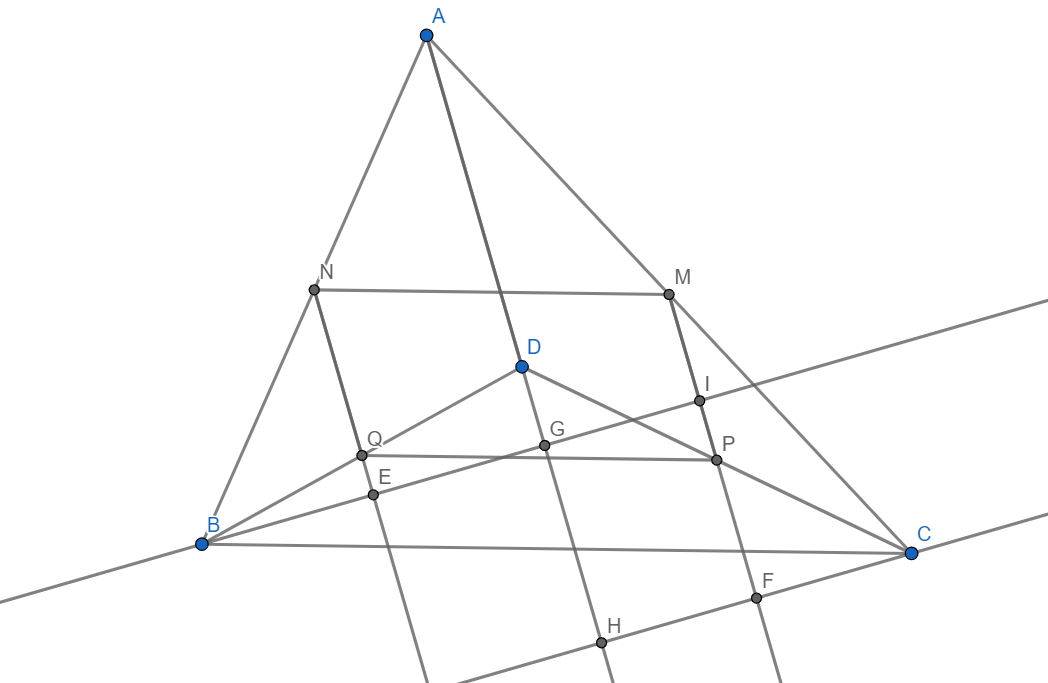
\includegraphics[scale=0.6]{IntermediateQ1_Day2Graphic.png}
\end{center}
Let $E$ and $G$ be the intersection of the lines $NQ$ and $AD$ with the perpendicular line from $B$ and $F$ and $H$ be the intersection of the lines $MP$ and $AD$.

By the midpoint theorem in $\triangle ABC$ and $\triangle BDC$ we have that $NM \parallel BC \parallel QP$, as well as midpoint theorem in $\triangle ABD$ and $\triangle ACD$, we find that $ON \parallel AD \parallel PM$ and $ON = \frac{AD}{2} =MP$. Thus, $NMPQ$ is a parallelogram. 

From $N$ being the midpoint of $AB$ and $ON||AD$, we have $BE = EG$ (midpoint theorem).
$M$ is the midpoint of $AC$ and $MP \parallel AD$ gives $HF = FC$.

Notice that since $AH \parallel MP$ and $BI \parallel CH$, we have $GI \parallel HF$ and $GH \parallel IF$ and thus, $GIFH$ is a parallelogram. Meaning that $GI = HF$.
From the above, we have:
\begin{align*}
Area(ABDC)
  & = Area(ABD) + Area(ACD) = \frac{BG \times AD}{2} + \frac{CH \times AD}{2} \\
  & = \frac{2EG \times AD + 2HF \times AD}{2}\\
  & = (EG + HF) \times AD = (EG + GI) \times AD\\
  & = EI \times AD = EI \times (2ON) = 2(EI \times ON) = 2 \times Area(NMPQ).
\end{align*}


\item % 2022, Andrew
Find all functions $f:\mathbb{R}\to\mathbb{R}$ such that:
\[f(x) + f(y) = f(2x+y) - x\] for all $x,y\in\mathbb{R}$.

\textbf{Solution:}
$y = -x$ gives us $f(x) + f(-x) = f(2x-x) - x \implies f(-x) = -x \implies f(x) = x$.
The check is trivial.

\item 
Find all $m,n\in \mathbb{Z}$ satisfying the following equation:
\begin{align}
m^3 + n^3 = (m+n)^2 
\end{align}

\textbf{Solution:} Notice that $m^3 + n^3$ can be factorised as $m^3 + n^3=(m+n)(m^{2} -mn + n^{2})$, thus we get:
\begin{align*}
    (m+n)(m^{2} -mn + n^{2}) & = (m+n)^2\\
    (m+n)(m^{2} -mn + n^{2} -m -n) & = 0.
\end{align*}
Thus, either $m = -n$ or $m^{2} -mn + n^{2} -m -n = 0$. The former is clearly a solution, so we consider the latter case henceforth. Observe that one can make the following factorisation:
\begin{align}
    m^{2} -mn + n^{2} -m -n & = 0 \nonumber\\ 
    m^{2} - mn + \frac{n^{2}}{4} + \frac{3n^{2}}{4} - m -n & = 0 \nonumber\\
    \left(m - \frac{n}{2}\right)^{2} - \left(m - \frac{n}{2}\right) + \frac{3n^{2}}{4} - \frac{3n}{2} & = 0 \nonumber\\
    \left(m - \frac{n}{2}\right)^{2} - \left(m - \frac{n}{2}\right) + \frac{1}{4} + \frac{3n^{2}}{4} - \frac{3n}{2} + \frac{3}{4} & = \frac{1}{4} +\frac{3}{4} \nonumber\\
    \left(m - \frac{n}{2} - \frac{1}{2}\right)^{2} +3\left(\frac{n}{2} - \frac{1}{2}\right)^{2} & = 1 \nonumber\\
    (2m - n - 1)^{2} + 3(n-1)^{2} & = 4 
\end{align}

If $(n-1)^{2} \geq 2$, we have
\begin{align*}
    3(n-1)^{2} & \geq 6 \\
    (2m - n - 1)^{2} & \geq 0 \\
    \Rightarrow 4 = (2m - n - 1)^{2} + 3(n-1)^{2} & \geq 6
\end{align*}
Which is not possible, thus $(n-1)^{2} \leq 1$. So we have either $(n-1)^{2} = 1$ or $(n-1)^{2} = 0$.
\begin{enumerate}
  \item If $(n-1)^{2} = 1$: $n = 2$ or $n=0$.
  \begin{enumerate}
    \item If $n=2$, then $(2)$ becomes $(2m -3)^{2} + 3 = 4 \implies 2m - 3 = 1$ or $2m - 3 = -1$. Thus $(m, n) = (2, 2), (1, 2)$.
    \item If $n = 0$, $(2)$ becomes $(2m -1)^{2} + 3 = 4 \implies 2m- 1 = 1$ or $2m - 1 = -1$, yielding $(m, n) = (1, 0), (0, 0)$.
  \end{enumerate}
  \item If $(n-1)^{2} = 0$: $n = 1$, then (2) becomes $(2m - 2)^{2} = 4$. Thus $(m, n) = (2, 1), (0, 1)$.
\end{enumerate}

\item % 2022, Emile
William and Beatrice take turns placing Kings on a $n \times m$ chessboard.
Kings cannot be placed on any of the 8 adjacent squares of Kings of \emph{differing} colour.
With William playing first as white, and Beatrice playing second as black, who has the winning strategy?

\textbf{Solution:} William will always have a winning strategy. William's first move is to place his initial king on a square that either contains the center-point or has the center-point of the board on its border. William can then rotate Beatrice's moves $180^{\circ}$ through the center-point of the board. Note that Beatrice cannot place a king in such a way that the reflection of her move is within the $8$ adjacent squares of the placed king. Therefor William will always be able to make a move as any legal move Beatrice plays will also have to be legal for William to play on the reflection. As the game is forced to end in less than $nm$ moves, William will place the last piece and have the winning strategy.


\item % Baltic Way 1994
In $\triangle ABC$ let $\angle C = 90^\circ$, and let $\Gamma$ be the circle with diameter $AC$. Define points $D$ and $E$ on $\Gamma$ such that $D$ is on $BC$ and $DE \parallel AC$. Let $P$ be the intersection of $AE$ and $BC$. Prove
\begin{flalign*}
  PC \cdot BC = AC^2.
\end{flalign*}

\textbf{Solution:} Notice that the statement is true if $\triangle ABC \mathop{|||} \triangle PAC$, but $\angle PCB = \angle ACB$ so the problem is reduced to showing that $\angle ABC = \angle PAC$. We have that
\begin{flalign*}
&& \angle ABC &= 90^\circ - \angle CAB  & (\angle's \text{ in } \triangle)\\
&& &= 90^\circ - (180^\circ - \angle ADE)  & (\text{co-int } \angle's)\\
&& &= 90^\circ - \angle ECA  & (\text{opp } \angle's\text{ cyc. quad}).
\end{flalign*}
But $AC$ is the diameter of $\Gamma$ so $\angle AEC = 90^\circ$ by Thales' Theorem. Therefore
\begin{flalign*}
  \angle ABC = 90^\circ - \angle ECA = \angle CAE = \angle PAC.
\end{flalign*}

\end{enumerate}

\end{document}
